\documentclass[DM,lsstdraft,toc]{lsstdoc}

\usepackage[english]{babel}
\usepackage[utf8x]{inputenc}
\usepackage{amsmath}
\usepackage{graphicx}
\usepackage{longtable}
\usepackage{hyperref}
\usepackage{comment}
\usepackage{natbib}

\excludecomment{changelog}
\excludecomment{todo}
\excludecomment{openissues}

% Local commands go here
\newcommand{\G}[1]{{\color{green} #1}}
\newcommand{\B}[1]{{\color{blue} #1}}
\newcommand{\R}[1]{{\color{red} #1}}

%% Journal abbreviations
\bibliographystyle{aasjournal}

\title[LSST Science Platform]{LSST Science Platform Vision Document}

\author{
M.~Juri\'c,
D.~Ciardi,
and
G.P.~Dubois-Felsmann
}

\setDocRef{LDM-nnn}
\date{\today}
\setDocRevision{1.0}
\setDocStatus{draft}

\setDocAbstract{%

This document defines the high-level vision for the {\bf LSST Science
Platform (LSP)}, a set of web applications and services through which the
the scientific community will to access, visualize, interact with,
and analyze LSST data holdings.
\\

It is meant to inform the development of requirements, product specifications,
prioritization, and plans for the Agile development of elements of the DM system 
that together make up the LSP.

}

% Change history defined here. Will be inserted into
% correct place with \maketitle
% OLDEST FIRST: VERSION, DATE, DESCRIPTION, OWNER NAME
\setDocChangeRecord{%
\addtohist{1}{2017-03-15}{Initial high-level description of the concept}{Mario Juric}
%\addtohist{2}{yyyy-mm-dd}{Future changes}{Future person}
}

\begin{document}

% Create the title page
% Table of contents will be added automatically if "toc" class option
% is used.
\maketitle

\section{Preface}

The purpose of this document is to lay out the high-level vision for the {\bf LSST Science Platform (LSP)}, a set of web applications and services through which the the scientific community will to access, visualize, interact with, and analyze LSST data holdings. With its companion document -- the Data Products Definition Document (\DPDD) -- it defines the high-level vision for LSST's end-user deliverables.
\\

To a future LSST user, this document should illustrate what will be made available to the science community through the LSST Data Access Centers. To LSST builders, it provides direction on how to flow down the LSST System Requirements Document to system design, sizing, budget and schedule as they pertain to the end-user services provided at the LSST Data Access Centers.
\\

Though under strict change control\footnote{LSST Docushare handle for this document is {\tt LSE-XXX}.}, this is a {\bf \em living document}. LSST will undergo a period of construction  and commissioning lasting no less than seven years, followed by a decade of survey operations. To ensure their continued scientific adequacy, the high-level vision for LSST Science Platform will be periodically reviewed and updated.

\clearpage

\section{Introduction}

\subsection{Goals and Philosophy}

The LSST is a facility whose primary mission is to acquire, process, and
make available the data collected by its telescope and camera, as well as
enable ``next-to-the-data'' creation of added-value (Level 3) data products
(\SRD).

This document describes the vision for the services to be put into place to
fulfill the ``{\em making available}'' and ``{\em Level 3} creation``
aspects of LSST's mission; its aim is to present a high-level
description of the data access and analysis services provided at the
LSST Data Access Centers. It should be read in conjunction with the
LSST Data Products Definition Document (\DPDD), which provides the high-level
description of LSST data products.

\subsection{LSST Science Platform Overview}

\begin{figure}
\centering
\scalebox{0.4}{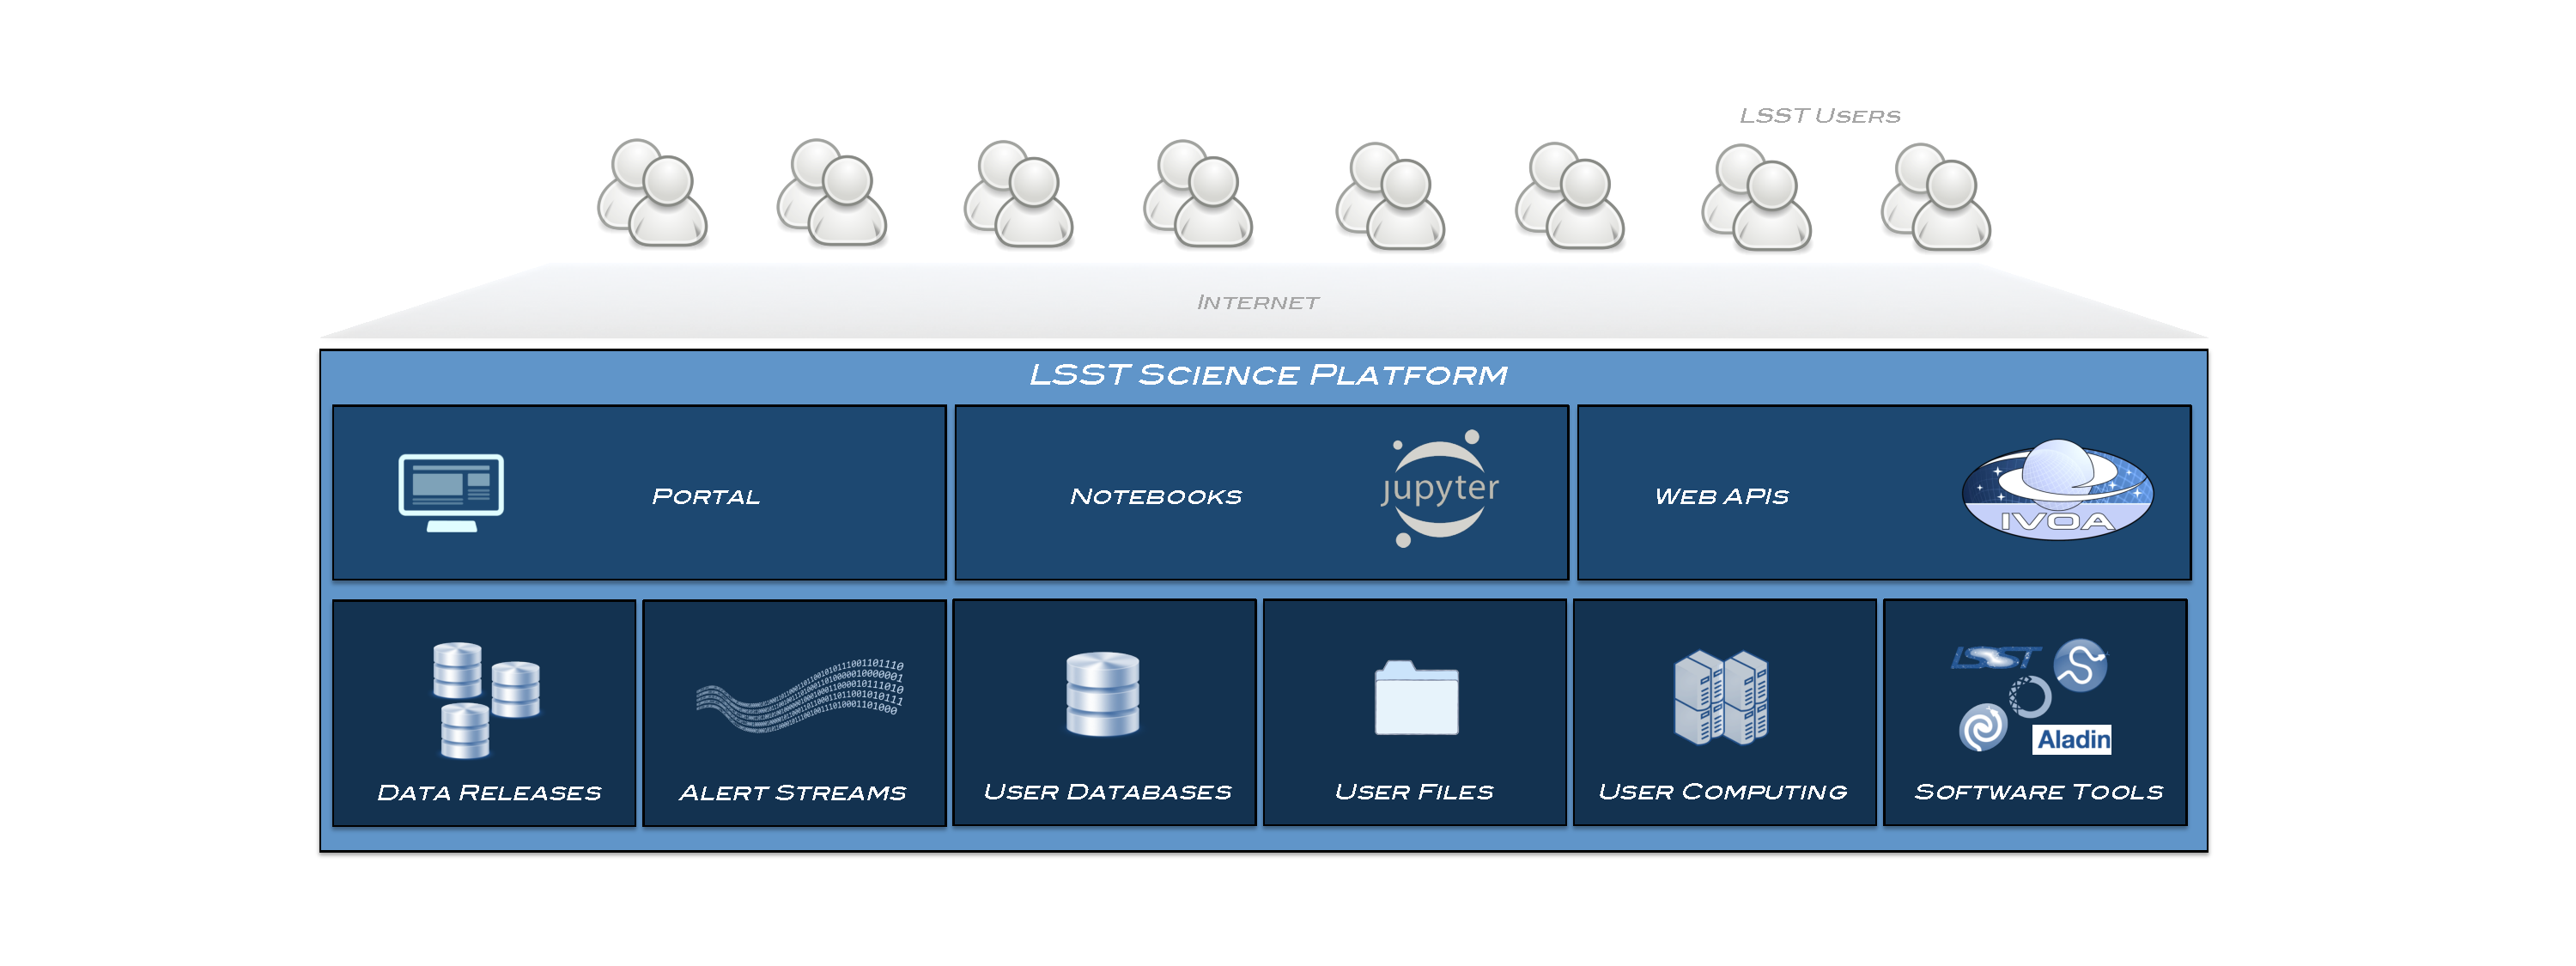
\includegraphics[trim={5cm 0.5cm 3cm 0.5cm},clip,page=1]{images/fig-lsst-science-platform-extended.pdf}}
\caption{
A high-level, layered, view of the LSST Science Platform.  The LSST data
will be exposed to the users through the web Portal, the Jupyter Notebook
interface, and machine-accessible Web APIs.  The web Portal component will
provide the essential data access and visualization services common to
present day archives.  The Notebook component, based on the Jupyter family
of technologies (JupyterHub and JupyterLab) will allow for more
sophisticated next-to-the-data analysis.  These user-visible services will
provide acces to the underlying core LSST data sets -- the data releases and
alert streams -- and be supported by the user Database, File Storage,
Computing, and Software Tools components.  Together, they will enable the
users to access, sub-select, analyze, and perform added-value processing of
all flavors of LSST Data Products (see text for detail). 
\label{fig:layeredLSP}}
\end{figure}

We define the {\bf LSST Science Platform as a set of web applications and services
made available to the scientific community to access, visualize, subset, and
perform next-to-the-data analysis of the LSST data set.}  The platform exposes the LSST data
and services to the user through three primary user-facing {\it aspects} -- the web {\bf Portal},
the {\bf JupyterLab} analysis environment, and a machine-accessible {\bf Web API} interface. These aspects provide three different way to access the data sets and analysis services provided in the LSST Data Access Centers (Figure~\ref{fig:layeredLSP}).

The {\bf Portal} aspect is a web portal designed to provide the essential data
access and visualization services through a simple-to-use website.  It will
enable browsing and visualization of the available datasets in ways the
users are accustomed to at archives such as IRSA, MAST, or the SDSS archive.

The {\bf JupyterLab} aspect will provide a Jupiter Notebook-like interface, and 
is geared towards enabling next-to-the-data analysis. The user experience will 
be nearly identical to working with Jupyter notebooks locally, except that computation
and analysis will occur at resources provided at the LSST Data Access Center.  This is an
implementation of the “bringing computation to the data” paradigm: rather
than imposing the burden of downloading, storing, and processing (large)
subsets of LSST data at their home institutions, we will enable our users to
bring their codes and perform their analysis at the LSST DAC.  We expect
this will reduce the barrier to entry and shorten the path to science for
the LSST science community.

The third, {\bf Web API}, aspect of the LSST Science Platform will expose the
services offered by the LSST Data Access Centers to other software tools and
services using commonly accepted protocols (e.g. industry-standard protocols
such as WebDAV, or Virtual Observatory protocols such as TAP or SIAP). This
interface will open the possibility for remote access and analysis of the LSST 
data set using well-known applications such as TOPCAT or libraries like AstroPy.

Finally, the LSST Science Platform is being envisioned to enable and encourage
collaborative work.  The capabilities ranging from sharing of derived
datasets within smaller groups, collaborations, or with the broader LSST
community, to collaborative visualization and editing capabilities expected
to become available within the JupyterLab ecosystem.

\section{User-facing Services}

\subsection{Web Portal}

\begin{figure}
	\centering
	\scalebox{0.4}{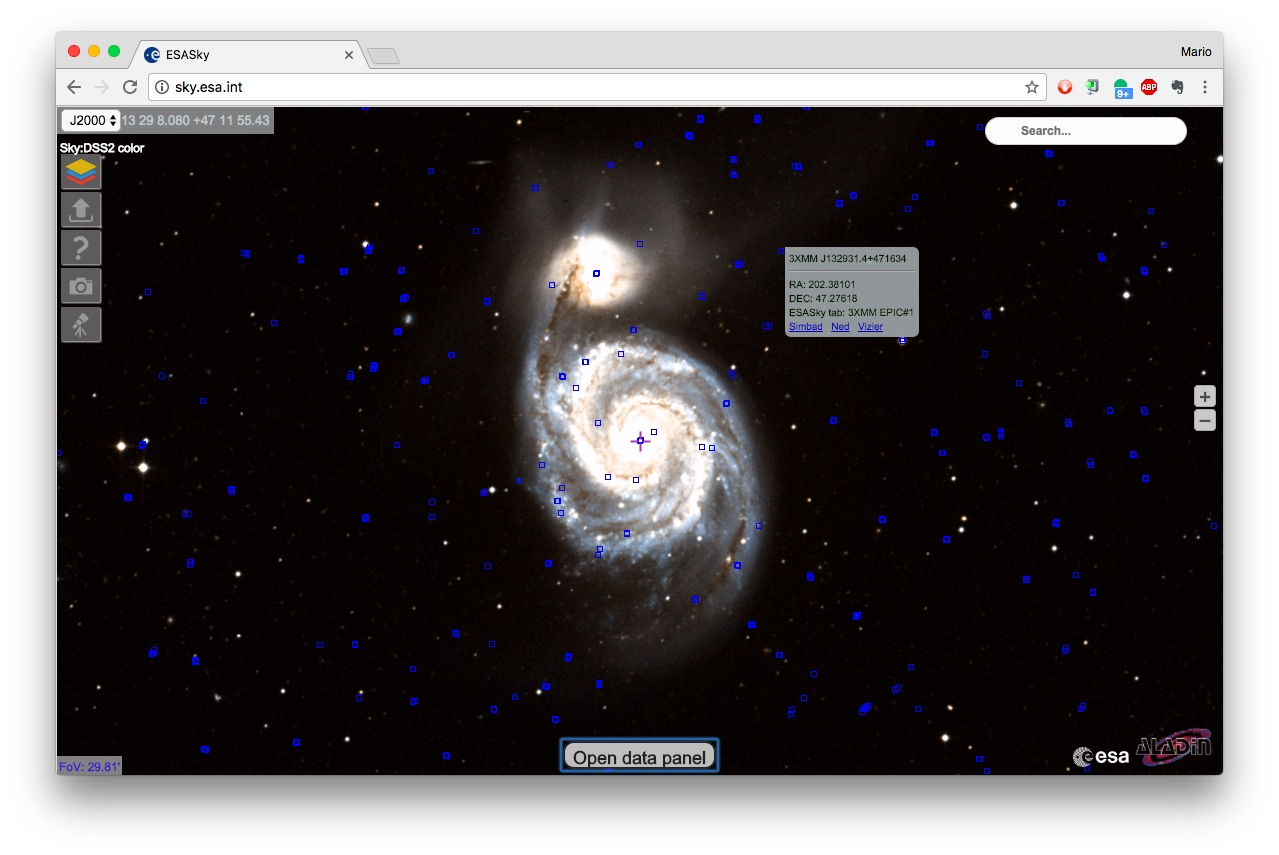
\includegraphics{images/fig-portal-esasky}}
	\caption{The "ESA Sky" web portal interface to ESA Archive holdings. The LSST portal user
		experience will support similar modern pan/zoom/select metaphor for exploration and visualization of the LSST data set.
		\label{fig:portalESA}}
\end{figure}

\begin{figure}
	\centering
	\scalebox{0.4}{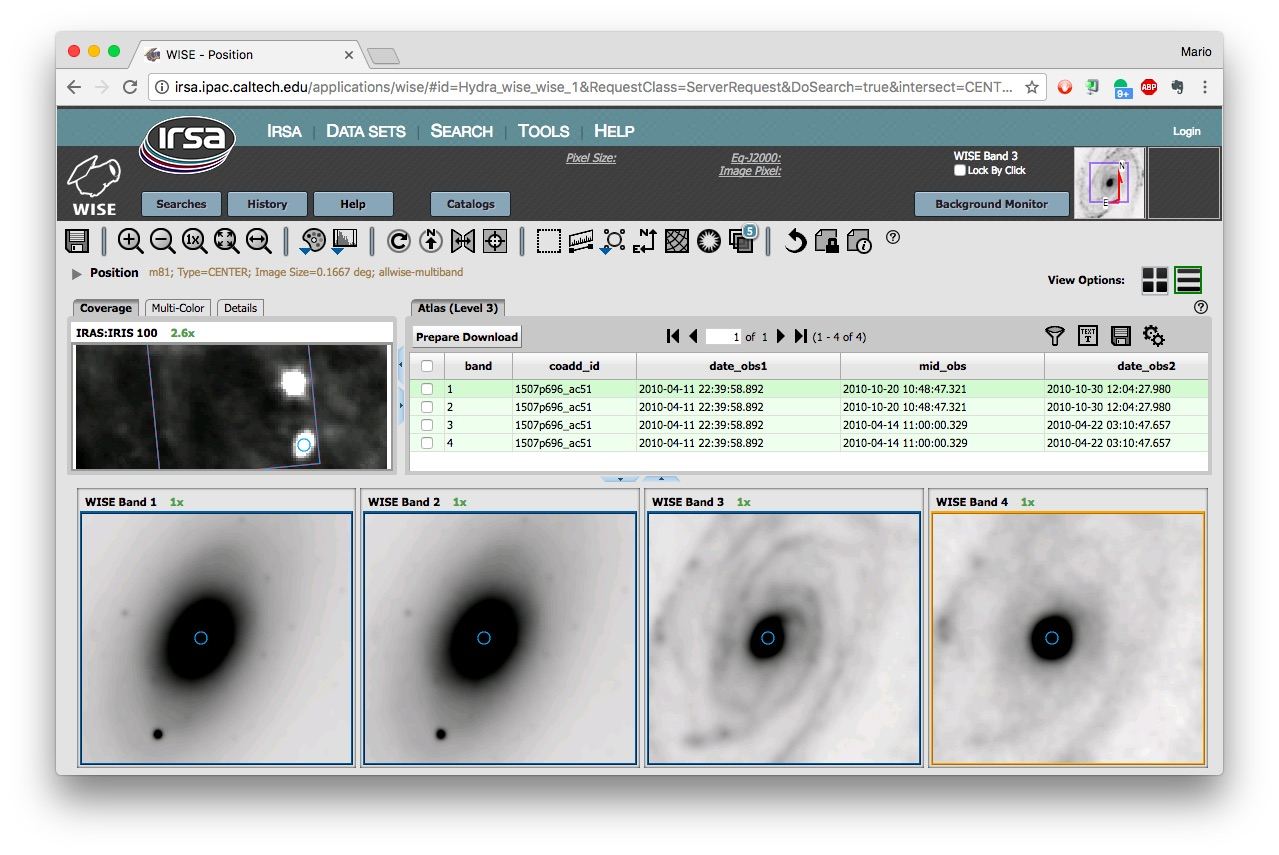
\includegraphics{images/fig-portal-irsa}}
	\caption{The web portal interface to the WISE data set at the Infra-Red Science Archive at IPAC. The LSST portal is being built by extending the Firefly toolkit that powers the IRSA/WISE archive.
		\label{fig:portalIRSA}}
\end{figure}

The {\bf Portal} aspect is a web portal designed to provide the essential data
access and visualization services through a simple-to-use website.  It will
enable browsing and visualization of the available datasets in ways the
users are accustomed to at archives such as IRSA, MAST, or the SDSS archive,
with an enhanced level of interactivity in line with expectations for
then-contemporary archive portals (similar to that found in ESASky and 
the DECaLS Viewer). Examples of the types of user experiences to be offered
through the LSST portal are shown in Figures~\ref{fig:portalESA}~and~\ref{fig:portalIRSA}.

Through the Portal, the users will be
able to view the LSST images, request subsets of data (via simple forms or
SQL queries), store the results of such queries to their personal
workspaces, construct commonly requested plots, and generally explore the
LSST dataset in a way that allows them to identify and access (subsets of)
data required by their science case.

\subsection{JupyterLab}

\begin{figure}
	\centering
	\scalebox{0.4}{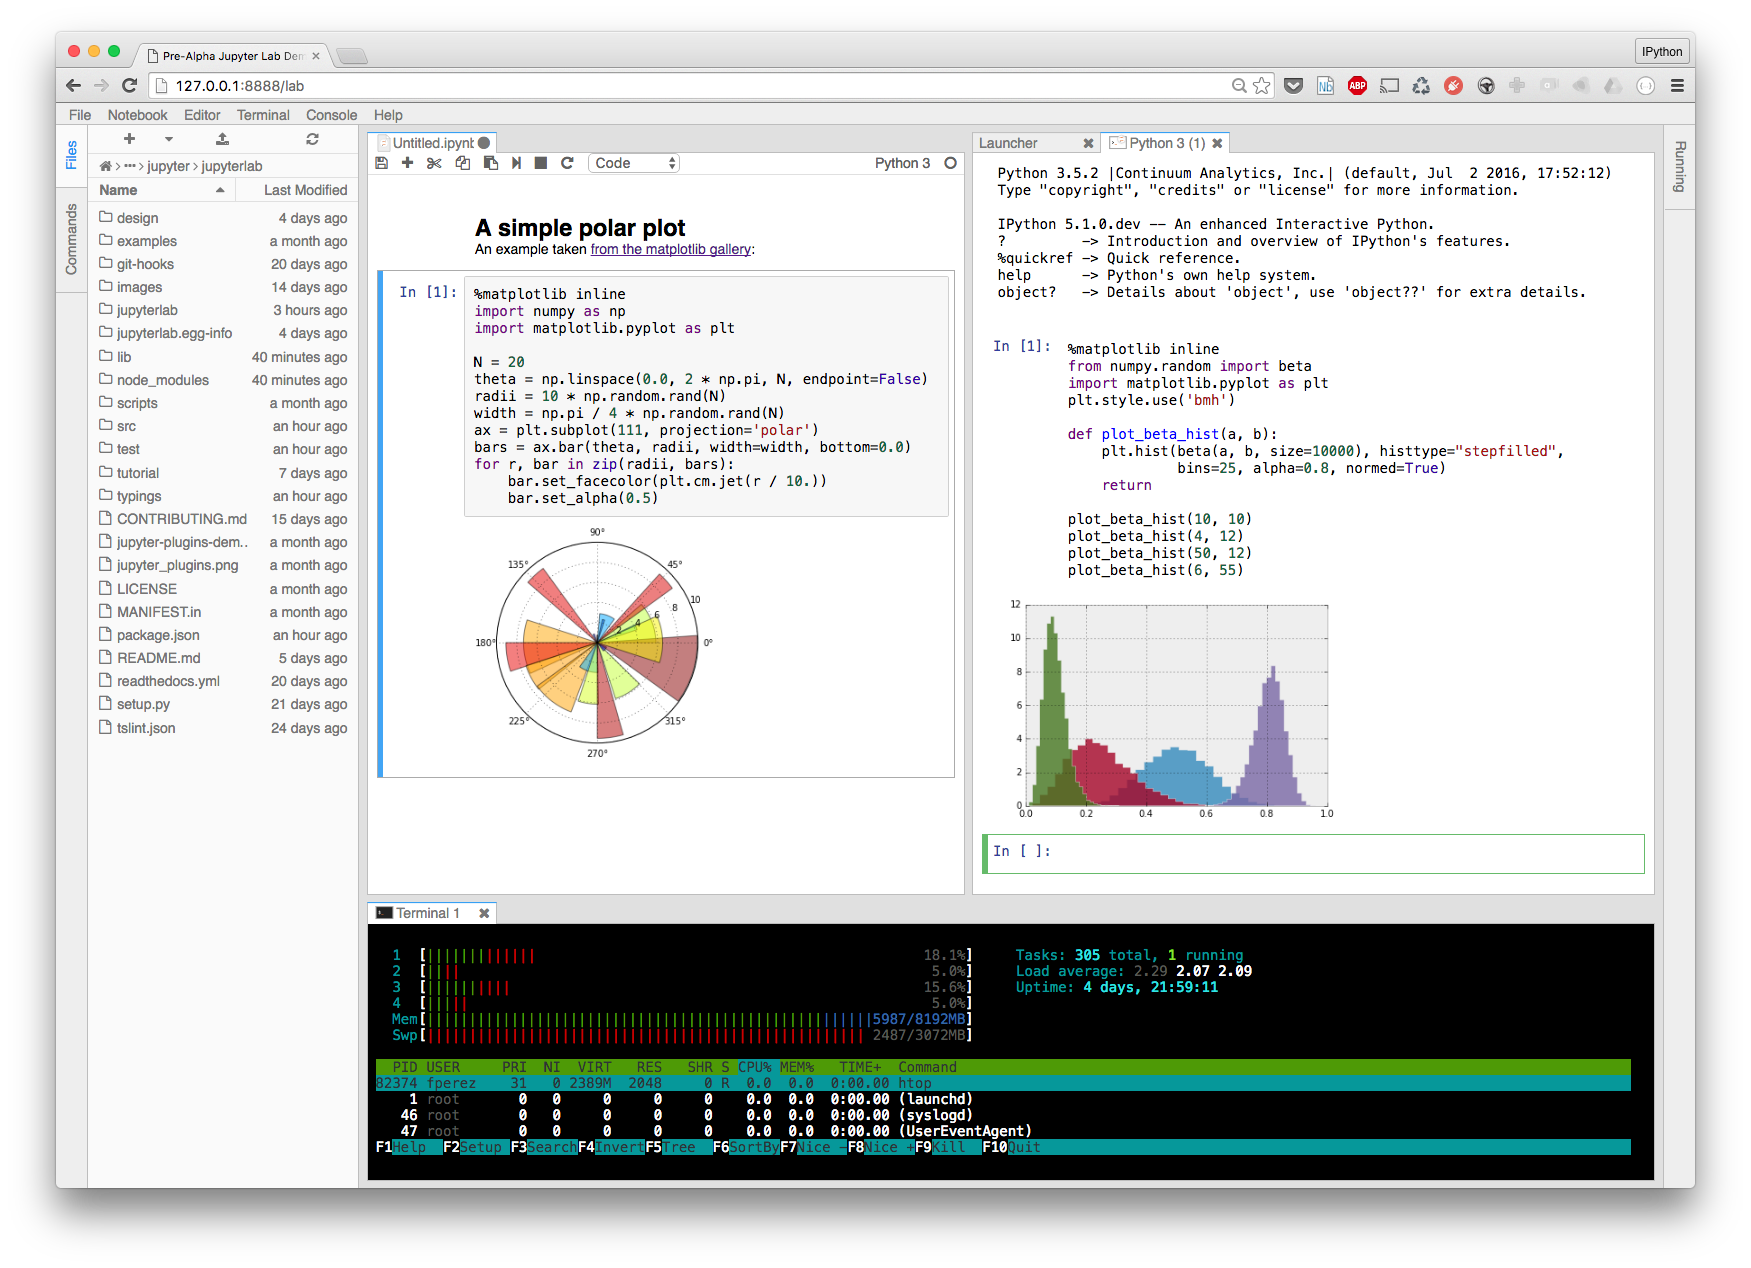
\includegraphics[scale=0.7]{images/jlab-screenshot-nb-con-term-2}}
	\caption{A screen capture of the JupyterLab interface (credit: JupyterLab team, \url{http://blog.jupyter.org/2016/07/14/jupyter-lab-alpha/})
		\label{fig:JupyterLab}}
\end{figure}

The {\bf JupyterLab} aspect, based on the Jupyter family of technologies (such as
JupyterHub and JupyterLab), will be provided to allow for more sophisticated
data selection, analysis, and creation of added value (Level 3) data
products. A screen capture of a mature prototype of JupterLab is shown in 
Figure~\ref{fig:JupyterLab}.

This environment will come preinstalled with a library of
commonly used and useful software Tools (such as AstroPy, LSST software
stack, Anaconda Scientific Python Distribution, and others).  The users will
be able to upload and install their own tools as well.

The JupyterLab user experience will be nearly identical to working with
Jupyter notebooks locally, except that computation and analysis will occur
at resources provided at the LSST Data Access Center.  This is an
implementation of the “bringing analysis to the data” paradigm: rather
than imposing the burden of downloading, storing, and processing (large)
subsets of LSST data at their home institutions, we will enable our users to
bring their codes and perform their analysis at the LSST DAC.  We expect
this will reduce the barrier to entry and shorten the path to science for
the LSST science community.

Add something about writing glue code to make it easy to submit jobs,
and how Notebooks will be the primary user interface to the backend batch system...

The JupyterLab aspect of the science platform will play a key role in commissioning,
quality assessment, and science validation of the as-built system. It will be the primary
method of performing interactive analysis of acquired data (e.g. adjusting and executing
prepared notebooks driving commissioning tasks), as well as commanding
the batch resources to execute larger processing tasks.

% Data sets acquired during commissioning, as well as precursor and simulated data sets processed for quality assessment and science validation while construction is ongoing, will appear in the commissioning workspace, ready for operator analysis using tools and

\subsection{Web APIs}

Backend Science Platform services (including access to
databases, images, and other files) will be exposed through
machine-accessible web APIs serving community-accepted formats and
protocols.  This will make it easy to initiate remote computations operating
on LSST data.  Virtual Observatory interfaces will allow connection to other
archives and enable the use of standard tools such as TOPCAT or DS9. 
This will further lower the barrier to access to LSST data, shortening the
path to science.

\begin{figure}
	\centering
	\scalebox{0.4}{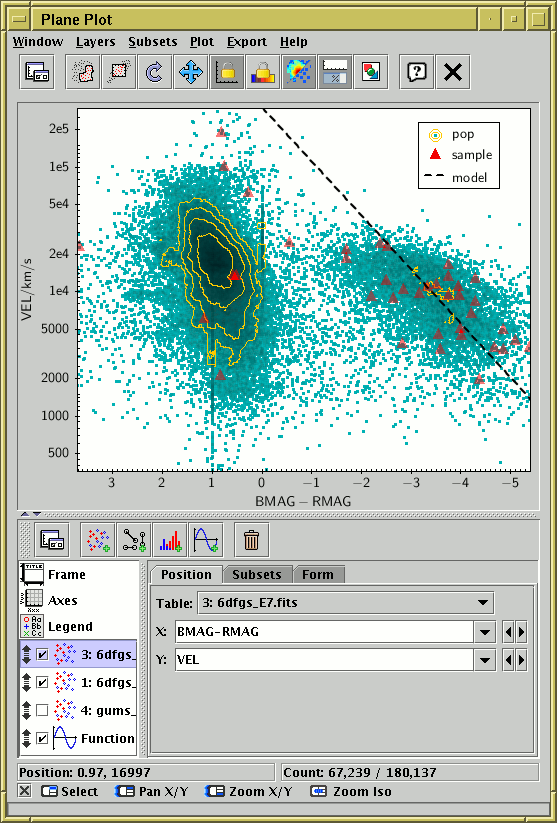
\includegraphics[scale=0.7]{images/topcat-StackPlotWindow}}
	\caption{A screen capture of Tool for OPerations on Catalogues And Tables (TOPCAT), that is capable of remotely accessing catalogs and images using VO protocols. Tools such as these will be able to directly access the data sets served by the LSST DACs (figure credit: Mark Taylor, \url{http://www.star.bris.ac.uk/~mbt/topcat/sun253/sun253.html}).
		\label{fig:toolsTOPCAT}}
\end{figure}

\subsection{Integrated environment}

All aspects of the Platform are intended to be {\it well integrated}, enabling a seamless workflow for the users to be able to move back and forth between them as needs dictate.  Our goal is to enable a user to find or create data in one aspect, and view or analyze that data in another.

As an example of how these connections can aid a user in exploring the LSST data, data queries will be shareable across the Portal and JupyterLab. This will allow a user to build a query using the Portal user interface, view the (possibly initial) results by browsing it in the Portal, and then access the final results from JupyterLab or a remotely connected client (e.g. TOPCAT) for further analysis. The reverse flow will also be enabled; a user can code and submit a complex SQL query in the Notebook and then browse and visualize the results in the Portal.

\subsection{Supporting Collaborative Work}

The LSST Science Platform will allow for collaborative work at two levels:
\begin{itemize}
	\item {\bf Workspaces}: Creation and sharing of data sets -- catalogs, images, queries, and other data products -- within a pre-defined group (eg., a research group at a University, or a large science collaboration). Such groups would have access to a shared virtual ``workspace'' within the LSST DAC, within which they can share file and catalog assets as well as allocated computing cycles. This shared workspace will be equally ``visible'' from all three aspects of the platform.
	
	\item {\bf Shared editing}: We expect to offer a ``Google Docs''-like collaborative editing, visualization, and data analysis capabilities. These are expected to become available within the Jupyter ecosystem, and will be included in the JupyterLab aspect as they do.
\end{itemize}

The levels of support for collaboration described above responsive to the large majority of user needs identified by end-user focus groups in R\&D. At the same time, they minimizing the technical risks by leveraging widely used and well understood technologies (SDSS MyDB-like user databases, backend A\&A mechanisms, VO protocols, Jupyter).

\section{Backend Services}

** UNFINISHED **

While 

\subsection{Serving Level 1 and 2 Data Products}

** UNFINISHED **

All data products will be made available using user-friendly databases and web services. More

In this section, we describe the high-level concepts for services used to serve the LSST catalogs and the event alert stream. Further details of the LSST data products may be found in the LSST Data Products Definition Document (\DPDD).

\section{Enabling Level 3: User Databases, File storage, and Computing}

** UNFINISHED **

--Need to say something about a batch system and MyDB type functionality being 
available to the user. May want to move some of the below discussion to
JupyterLab section? Is this the place to introduce the Workspace concept?--

Queries, visualizations, and analysis performed through the Portal and
Notebooks will be served by a shared computing cluster, file storage, and
database resource (bottom row of Figure~\ref{fig:layeredLSP}).  At start of operations,
this computing cluster will number 2,400 cores (approximately 18 TFLOPs),
with 4 PB of file and 3 PB of database storage (numbers for the U.S.  DAC). 
These will be shared by all users, the number of whom we’re estimating in
the low thousands.

Not all users will be accessing the computing cluster concurrently; though
difficult to predict with accuracy because of a lack of direct comparables,
an estimate on order of a ~100 concurrent users is likely reasonable.  This
would translate to typical allocations of ~20 cores per user, sufficient to
enable preliminary end-user science analyses (working on catalogs, smaller
number of images) and creation of some added-value (Level 3) data products. 
A good analogy is one of being given a server with a few TB of disk, few TB
of database storage, that is co-located next to the LSST data, and with a
chance to use tens to hundreds of cores for analysis (depending on system
load).

For larger endeavors (e.g., pixel-level reprocessing of the entire LSST
dataset), the users will be steered towards resources beyond the LSST DACs
(e.g., national supercomputing centers, university computing centers, or the
public cloud).

\section{Development Methodology and Prioritization Guidance}

\subsection{Iterative Development Leveraging Existing Technologies }

The services constructed for the LSST Science Platform will be developed following the iterative, Agile methodology. This is especially desirable for user-facing services, where iterative development and nearly continuous stakeholder feedback provide guidance as to the details of features to be implemented, and the delivery of intermediate milestones.

The development of the LSP Portal. JupyterLab, as well as Web API aspects will start from significant existing code bases, standards, and prior art. This is a deliberate approach designed to minimize risk, and leverage end-user familiarity with these interfaces, thus reducing the barrier to adoption of the interface eventually deployed for LSST.

The {\bf Portal} is based on existing, production quality, archive portal interface developed at IRSA/IPAC -- the {\em Firefly} toolkit. The primary challenge is integrating the existing Firefly code, and updating the user experience to conform to anticipated user expectations (e.g., supporting all-sky maps and pan/zoom/click-type exploration). Consistent with the general philosophy, DM should look at achieving the necessary upgrades by re-using existing well-known tools and libraries (e.g. Aladin Lite).

Similarly, the {\bf JupyterLab} environment will be based on the open-source JupyterLab product delivered and maintained by the Juptyter team. The development of the JupyterLab aspect of the LSST Science Platform should focus on deployment and integration with the backend services and other aspects of the platform, rather than developing new or radically different features within the JupyterLab product.

Finally, the {\bf Web API} aspect is envisioned as implementing existing, widely-adopted, community protocols (e.g. such as those from Virtual Observatory suite of protocols and standards), down to leveraging existing libraries wherever appropriate.

\subsection{Prioritization Guidance}

Here we give some overall feature prioritization guidance, to enable the construction of initial (mostly functional) requirements and intermediate development milestones.

Portal aspect:
\begin{enumerate}
	\item Deployment of the initial Firefly back-end within the (prototype) LSST Data Access Center at NCSA.
	\item Integration of the initial Firefly front- and back-ends with the LSP backend services. For example, this includes the authentication and authorization mechanisms, relational databases, file stores, etc.
	\item User experience improvements, such as addition all-sky maps with pan/zoom/select navigation metaphors, modernization of the look-and-feel, streamlining of the UI and deprecation of rarely used widgets. {\bf Once this level of functionality is met (at scale), the Portal aspect will have achieved the minimum level of viability for deployment to operations}.
	\item Improved user workflow integration with other aspects of the LSST Science Platform. For example, it should be possible to begin data exploration in the Portal (e.g., by interactively selecting data sets) and seamlessly transfer the sub-selected catalogs and images to the JupyterLab environment for further, more complex, analysis using provided Python libraries.
	\item Addition of new new widgets and abilities to the Portal, that address most requested and broadly useful end-user needs.
	\item Widget-level integration with JupyterLab.
\end{enumerate}

JupyterLab aspect:
\begin{enumerate}
	\item Deployment of the initial JupyterLab product within the (prototype) LSST Data Access Center at NCSA.
	\item Integration of the JupyterLab product with LSP backend services, most notably authentication and authorization, user management, databases, and file stores. {\bf Once this level of functionality is met (at scale), the JupyterLab aspect will have achieved the minimum level of viability for deployment to operations}.
	\item Development of libraries and utilities to ease the submission of user-written code from Jupyter notebooks to the batch system.
	\item Creation and curation of a library of 3rd party code that will be made available to LSP end-users.
\end{enumerate}

Web APIs:
\begin{enumerate}
	\item Development and deployment of initial data access APIs needed to satisfy the back-end needs of the Portal and JupyterLab aspects. These may not yet "speak" the final, standards-compliant, protocols.
	\item Integration of the Web API aspect with LSP backend services, most notably authentication and authorization, user management, databases, and file stores. 
	\item Deployment of standards-compliant protocols throughout the Web API aspect, and integration with all other elements of the Platform. {\bf Once this level of functionality is met (at scale), the Web API aspect will have achieved the minimum level of viability for deployment to operations}.
\end{enumerate}

\end{document}
